\section{Ziel}
Das Ziel dieses Versuches ist es, mithilfe der Ablenkung
eines Elektronenstrahls im elektrischen sowie im transversalen
Magnetfeld bestimmte Eigenschaften zu untersuchen.
Dazu zählen die spezifische Elektronenladung, die Intensität
des Erdmagnetfeldes und die Proportionalität zwischen der
Verschiebung des Leuchtflecks des Elektronenstrahls und der
angelegten Ablenkspannung. Außerdem soll ein Kathodenstrahl-
Oszillograph untersucht werden.

\section{Theorie}
\label{sec:Theorie}
Für beide Versuchsteile wird eine Röhre verwendet, in der ein
Vakuum erzeugt wurde. Dafür wird die so genannte Kathodenstrahlröhre 
bis auf einen Restdruck von ca. $\SI{1e-6}{\milli\bar}$
evakuiert. 

\subsection{Theoretische Grundlage im elektrischen Feld}
%irgendwas hinschreiben

\subsubsection{Aufbau einer Kathodenstrahlröhre}
Eine Kathodenstrahlröhre besteht aus drei 
Teilen (siehe Abb. \ref{fig:roehre}). Im vorderen Teil der Kathodenstrahlröhre  werden in der sogenannten Elektronenkanone Elektronen erzeugt, beschleunigt und zu einem Strahl fokussiert. 
Anschließend werden sie von einem Ablenksystem, das aus elektrisch geladenen Platten besteht, in verschiedene Richtungen gelenkt, und im dritten Bereich von einer Vorrichtung auf einem Schirm visuell nachgewiesen. 
\begin{figure}
    \centering
    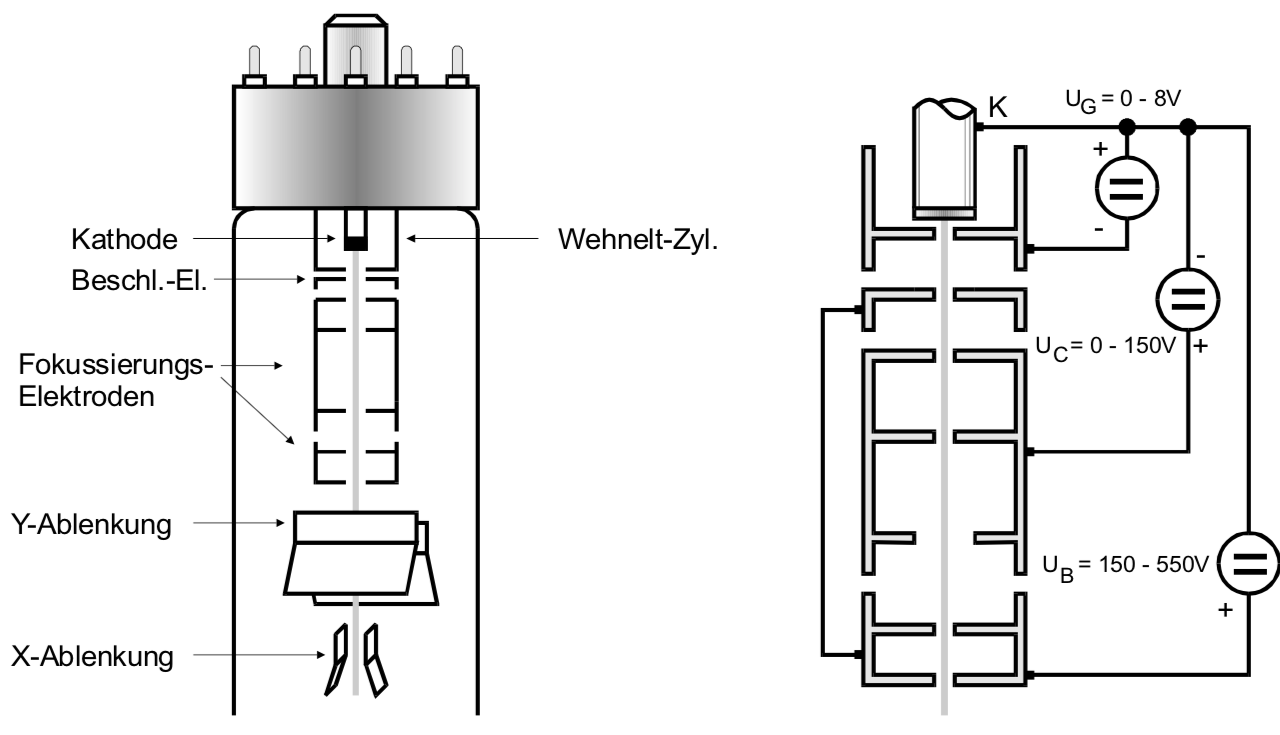
\includegraphics[width=12cm, height=7cm]{build/roehre.png}
    \caption{Der Aufbau einer Kathodenstrahlröhre. \cite{V501}}
    \label{fig:roehre}
\end{figure}

\noindent An einer Glühkathode werden die Elektronen durch eine Heizspannung, die an einem Draht anliegt, erzeugt.  
Diese ganze Apparatur befindet sich in einem Wehneltzylinder, der dafür da ist, dass der Nutzer über einen Drehknopf von außen die Intensität beeinflussen kann. Der Zylinder ist nämlich elektrisch negativ geladen und kann so genutzt werden, um die Elektronen zusätzlich zu beschleunigen und somit die Intensität zu steuern. 
%Durch das negativen Potential des Zylinders kann die Intensität 
%des Elektronenstrahls gesteuert werden. 
Als Gegenpol zu dem Wehneltzylinder gibt es ein Elektrode, die positiv geladen ist. Somit werden die Elektronen, die sich zwischen dem Zylinder und der dieser Elektrode befinden, zur dieser hin beschleunigt. Die Geschwindigkeit, die sie haben, nachdem sie den Zylinder verlassen konnten, beträgt $v_\text{z}$.  
Daraus ergibt sich dann mit dem Energiesatz  
\begin{equation}
    \frac{m_0 \, v_\text{Z}^2}{2} = e_\text{0} \, U_\text{B}.
    \label{eqn:energie}
\end{equation}

\noindent Hinter der Elektrode befinden sich weitere Elektroden, 
die dafür da sind, den Strahl zu fokussieren. Der gebündelte 
Strahl fällt am Ende der Apparatur auf einen Leuchtschirm, 
auf dem die auftreffenden Elektronen die Aktivatorzentren zur 
Emission von Lichtquanten anregen.
Der Leuchtschirm ist mit der Beschleunigungselektrode 
verbunden, sodass er sich nicht negativ laden kann.
Das Ablenksystem besteht aus zwei Plattenpaaren, deren Normalen 
senkrecht aufeinander stehen. Legt man eine Spannung an diese 
Platten an, übt das davon erzeugte $E$-Feld eine Kraft 
auf den Elektronenstrahl aus. 

\subsubsection{Berechnung der Ablenkung eines Elektronenstrahls im elektrischen Feld} %gleiche Überschrift wie in der Anleitung
Die folgenden Gleichungen können in Abb. \ref{fig:roehre2}
grafisch nachvollzogen werden.
\begin{figure}
    \centering
    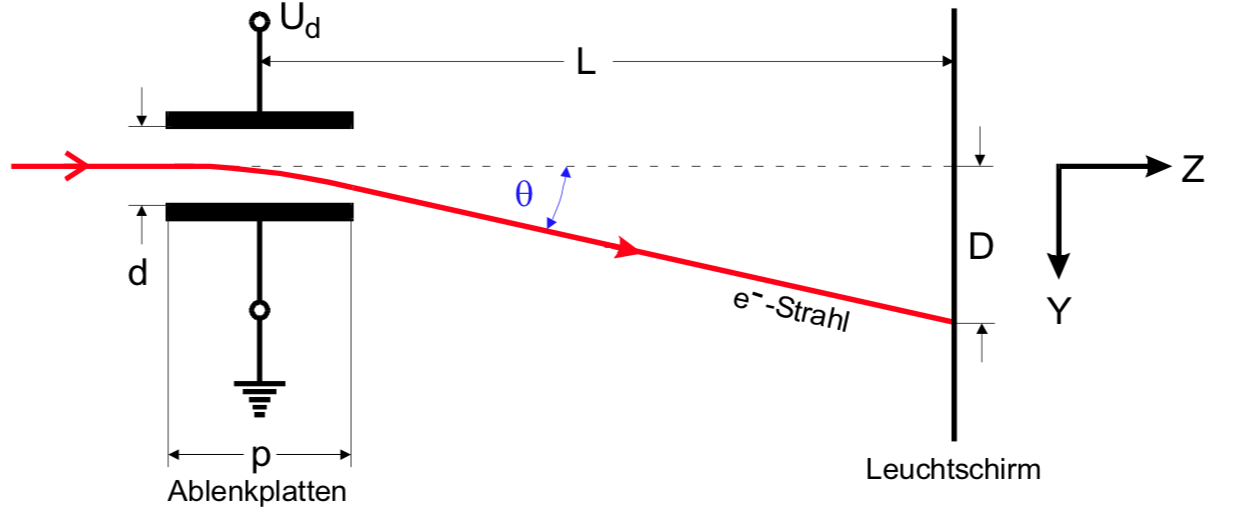
\includegraphics[width=12cm, height=6cm]{build/roehre2.png}
    \caption{Schematische Darstellung der Ablenkung des
    Elektronenstrahls in der Kathodenstrahlröhre. \cite{V501}}
    \label{fig:roehre2}
\end{figure}

\noindent 
Ein elektrisches Feld zwischen zwei Platten kann als homogen angenommen werden,
wenn der Abstand $d$ zwischen den Platten klein gegen die Länge $p$
der beiden Platten ist.
Aus dieser Näherung ergibt sich dann, dass die Feldstärke 
\begin{equation*}
    E = \frac{U_\text{d}}{d}
\end{equation*}
ist.
Auf ein Elektron wirkt dann die Coulombkraft, 
die außerhalb der Platten null wird im Rahmen dieser Näherung. Diese Kraft ist konstant, 
wodurch sich eine Beschleunigung in $y$-Richtung  
%---> wir haben vorher keine Richtungen erwähnt
ergibt. 
Die erreichte Geschwindigkeit ist 
\begin{equation*}
    v_\text{y} = \frac{e_\text{0}}{m_\text{0}} \frac{U_\text{d}}{d} \Delta t.
\end{equation*}

\noindent Mit der Plattenlänge und der 
gleichförmigen Geschwindigkeit $v_\text{z}$ ergibt sich $\Delta t$ zu
\begin{equation*}
    \Delta t = \frac{p}{v_\text{z}}.
\end{equation*}

\noindent Dieser Ausdruck kann in die vertikale 
Geschwindigkeit $v_\text{y}$ eingesetzt werden. Der Winkel $\theta$ der 
Richtungsänderung setzt sich aus der Division von 
$v_\text{y}$ durch $v_\text{z}$ zusammen. 

\noindent Damit ergibt sich für die Verschiebung $D$ des Leuchtflecks 
\begin{equation*}
    D = L \, \theta = \frac{e_\text{0}}{m_\text{0}} \, L \, \frac{U_\text{d}}{d} \frac{p}{v_\text{z}^2}.
\end{equation*}

\noindent Mit Gleichung \eqref{eqn:energie} ergibt sich dann 
\begin{equation}
    D = \frac{p}{2\, d} \, L \, \frac{U_\text{d}}{U_\text{B}}.
    \label{eqn:leuchtfleck}
\end{equation}

\subsubsection{Der Kathodenstrahl-Oszillograph}
Mit einem Kathodenstrahl-Oszillographen kann die Zeitabhängigkeit
von Wechselspannungen darstellt werden.
Dazu wird an das Plattenpaar, das den Strahl in horizontaler
Richtung ablenkt, eine Sägezahnspannung angelegt. An das Plattenpaar,
das den Strahl vertikal ablenkt, wird die zu untersuchende
Spannung angelegt. Wenn die Synchronisationsbedingung
\begin{equation*}
    n \, \nu_\text{Sä} = m \, \nu_\text{We}
\end{equation*}
erfüllt ist, wird der Verlauf der Wechselspannung auf dem
Leuchtschirm angezeigt.


\subsection{Theoretische Grundlage im magnetischen Feld}
Elektrische Felder üben auf ruhende Ladungen 
eine Kraft aus. Magnetostatische Felder dagegen üben nur auf 
Ladungen, die sich relativ zum Feld bewegen, eine Kraft aus.

\subsubsection{Berechnung der Elektronenbahn im homogenen Magnetfeld}
Die Lorentzkraft ist so definiert, dass sie auf eine bewegte Ladung $q$, die sich mit einer Geschwindigkeit $v$ in einem homogenen $B$-Feld bewegt, wirkt. Es gilt dann 
\begin{equation}
    \vec{F_\text{L}}= q \, \vec{v} \cross \vec{B}.
    \label{eqn:Lorentz}
\end{equation}

\noindent Durch das Kreuzprodukt ergibt sich, dass die senkrecht zum $B$-Feld bewegte Ladung eine maximale Kraft spürt, während eine parallel zum $B$-Feld bewegte Ladung gar keine Kraft erfährt.

\noindent Durch die Kraft des Magnetfelds ändert sich allerdings nur die Richtung der Ladung und sie ändert 
in der Theorie nicht die Geschwindigkeit. Also ist die Energie konstant 
innerhalb des Systems der Ladung.
%-> E_pot ändert sich nicht -> E_kin konstant -> |vec(v)|=v_0 konstant

\noindent Der Krümmungsradius $r$ lässt sich bestimmen, indem Lorentz- und der Zentrifugalkraft gleichgesetzt werden. Daraus folgt
\begin{equation}
    r= \frac{m_\text{0} \, v_\text{0}}{e_\text{0} \, B}.
    \label{eqn:radius}
\end{equation}
Die Krümmungsbahn ist eine Kreisbahn, weil der Radius
bei einer gegebenen Einstellung von $B$, und wenn die Geschwindigkeit $v_0$ der Elektronen bekannt ist, konstant ist. 

\subsubsection{Bestimmung der spezifischen Elektronenladung}

Die spezifische 
Ladung von Elektronen $e_\text{0}/m_\text{0}$ lässt sich
mit Gleichung \eqref{eqn:radius} bestimmen. 
Die konstante Geschwindigkeit $v_\text{0}$ ergibt sich zu 
\begin{equation*}
    v_\text{0}= \sqrt{2 \, U_\text{B} \frac{e_\text{0}}{m_\text{0}}}.
\end{equation*}
Dabei ist $U_\text{B}$ die Beschleunigungsspannung, die an dem Draht angelegt ist.

\noindent Sind alle Felder innerhalb der Kathodenstrahlröhre ausgeschaltet, wird ein Leuchtfleck in der Mitte des Schirms erzeugt werden.  
Wenn ein Magnetfeld in x-Richtung eingeschaltet wird, verschiebt sich 
der Leuchtfleck aufgrund der Krümmung auf der y-Achse 
um den Abstand $D$ nach oben oder nach unten. Zwischen dem Wirkungsbereich $L$ (das ist die Weite 
zwischen der Quelle und dem Schirm), der y-Verschiebung  $D$ und dem 
Radius $r$ ergibt sich über den Satz des Pythagoras der Zusammenhang 
\begin{equation*}
    r = \frac{L^2 + D^2}{2D}.
\end{equation*}
Dieser kann in \eqref{eqn:radius} eingesetzt werden.
Damit ergibt sich  
\begin{equation}
    \frac{D}{L^2 + D^2}= \frac{1}{\sqrt{8 \, U_\text{B}}}\sqrt{\frac{e_\text{0}}{m_\text{0}}} B,
    \label{eqn:Ende}
\end{equation}
womit die spezifische Ladungen durch eine Auftragung der linken und rechten Seite der Gleichung gegeneinander bestimmt werden kann. 

\subsubsection{Das Helmholtz-Spulenpaar}
Ein Helmholtz-Spulenpaar kann ein homogenes Magnetfeld erzeugen.
Der Radius $R$ beider Spulen entspricht dem Spulenabstand.
Die Windungszahl $N$ der Spulen ist ebenfalls identisch.
Im Mittelpunkt ist die Flussdichte $B$ durch
\begin{equation}
    B = \mu_0 \, \frac{8}{\sqrt{125}} \, \frac{N \, I}{R}
    \label{eqn:helmholtz}
\end{equation}
gegeben.

\subsubsection{Erdmagnetfeld}
Die Totalintensität des Erdmagnetfelds ergibt sich mit der horizontal Komponente $B_\text{horizontal}$ und dem Winkel $\varphi$ zu %horizontal oder vertikal und wie heißt der Winkel 
\begin{equation}
    B_\text{total} = \frac{B_\text{horizontal}}{\cos{\varphi}}.
    \label{eqn:btotal}
\end{equation}
